\documentclass[10pt]{beamer}
\usetheme[
%%% options passed to the outer theme
%    hidetitle,           % hide the (short) title in the sidebar
%    hideauthor,          % hide the (short) author in the sidebar
%    hideinstitute,       % hide the (short) institute in the bottom of the sidebar
%    shownavsym,          % show the navigation symbols
%    width=2cm,           % width of the sidebar (default is 2 cm)
%    hideothersubsections,% hide all subsections but the subsections in the current section
%    hideallsubsections,  % hide all subsections
%    left                % right of left position of sidebar (default is right)
  ]{Aalborg}
  
% If you want to change the colors of the various elements in the theme, edit and uncomment the following lines
% Change the bar and sidebar colors:
%\setbeamercolor{Aalborg}{fg=red!20,bg=red}
%\setbeamercolor{sidebar}{bg=red!20}
% Change the color of the structural elements:
%\setbeamercolor{structure}{fg=red}
% Change the frame title text color:
%\setbeamercolor{frametitle}{fg=blue}
% Change the normal text color background:
%\setbeamercolor{normal text}{bg=gray!10}
% ... and you can of course change a lot more - see the beamer user manual.

\usepackage[utf8]{inputenc}
\usepackage[spanish]{babel}
\usepackage[T1]{fontenc}
% Or whatever. Note that the encoding and the font should match. If T1
% does not look nice, try deleting the line with the fontenc.

%\usepackage[table,xcdraw]{xcolor}
\usepackage{helvet}
\usepackage{graphicx}
\usepackage{tikz}
\usetikzlibrary{shapes,arrows,positioning}

%\usepackage{minted}
\usepackage{listings}
\usepackage{color}
\definecolor{codegreen}{rgb}{0,0.6,0}
\definecolor{codegray}{rgb}{0.5,0.5,0.5}
\definecolor{codepurple}{rgb}{0.58,0,0.82}
\definecolor{backcolour}{rgb}{0.95,0.95,0.92}
 
\lstdefinestyle{mystyle}{
    backgroundcolor=\color{backcolour},   
    commentstyle=\color{codegreen},
    keywordstyle=\color{magenta},
    numberstyle=\tiny\color{codegray},
    stringstyle=\color{codepurple},
    basicstyle=\footnotesize,
    breakatwhitespace=false,         
    breaklines=true,                 
    captionpos=b,                    
    keepspaces=true,                 
    numbers=left,                    
    numbersep=5pt,                  
    showspaces=false,                
    showstringspaces=false,
    showtabs=false,                  
    tabsize=2
}
 
\lstset{style=mystyle}


% colored hyperlinks
\newcommand{\chref}[2]{%
  \href{#1}{{\usebeamercolor[bg]{Aalborg}#2}}%
}

\title[Servomecanismos]% optional, use only with long paper titles
{Servomecanismos}

%\title[Sensores y Actuadores]% optional, use only with long paper titles
%{Sensores y Actuadores}

%\title[Percepción]% optional, use only with long paper titles
%{Percepción}

\subtitle{Git y Github para poetas, parte 7}  % could also be a conference name

\date{\today}

\author[Víctor Medrano Zarazúa] % optional, use only with lots of authors
{
  Víctor Medrano Zarazúa\\
  \href{mailto:victor.medranozr@uanl.edu.mx}{{\tt victor.medranozr@uanl.edu.mx}}
}
% - Give the names in the same order as they appear in the paper.
% - Use the \inst{?} command only if the authors have different
%   affiliation. See the beamer manual for an example

\institute[
%  {\includegraphics[scale=0.2]{aau_segl}}\\ %insert a company, department or university logo
  %Dept.\ of Electronic Systems\\
  Universidad Autónoma de Nuevo León\\
  Facultad de Ingeniería Mecánica y Eléctrica
] % optional - is placed in the bottom of the sidebar on every slide
{% is placed on the bottom of the title page
  %Department of Electronic Systems\\
  Universidad Autónoma de Nuevo León\\
  Facultad de Ingeniería Mecánica y Eléctrica
  
  %there must be an empty line above this line - otherwise some unwanted space is added between the university and the country (I do not know why;( )
}

% specify the logo in the top right/left of the slide
\pgfdeclareimage[height=1cm]{mainlogo}{AAUgraphics/FIME} % placed in the upper left/right corner
\logo{\pgfuseimage{mainlogo}}

% specify a logo on the titlepage (you can specify additional logos an include them in 
% institute command below
\pgfdeclareimage[height=1.5cm]{titlepagelogo}{AAUgraphics/UANL} % placed on the title page
%\pgfdeclareimage[height=1.5cm]{titlepagelogo2}{AAUgraphics/aau_logo_new} % placed on the title page
\titlegraphic{% is placed on the bottom of the title page
  \pgfuseimage{titlepagelogo}
%  \hspace{1cm}\pgfuseimage{titlepagelogo2}
}

%\definecolor{UniBlue}{RGB}{255,255,255}

\tikzset{
block/.style={
  draw, 
  fill=blue!20, 
  rectangle, 
  minimum height=3em, 
  minimum width=6em
  },
 gain/.style={
    draw,
    fill=blue!20, 
    isosceles triangle,
    minimum height = 3em,
    isosceles triangle apex angle=60
    },
sum/.style={
  draw, 
  fill=blue!20, 
  circle, 
  },
input/.style={coordinate},
output/.style={coordinate},
pinstyle/.style={
  pin edge={to-,thin,black}
  }
}  

\newcommand{\heart}{\ensuremath\varheartsuit}
\newcommand{\butt}{\rotatebox[origin=c]{180}{\heart}}

\begin{document}
% the titlepage


%\setbeamercolor{title}{fg=UniBlue}
%\setbeamercolor{normal text}{fg=UniBlue}
%\setbeamercolor{Aalborg}{fg=black,bg=black}


{\aauwavesbg
\begin{frame}[plain,noframenumbering] % the plain option removes the sidebar and header from the title page
  \titlepage
\end{frame}}
%%%%%%%%%%%%%%%%

% TOC
\begin{frame}{Contenido}{}
\tableofcontents
\end{frame}
%%%%%%%%%%%%%%%%
\section{Repaso}
\begin{frame}{Repaso}{}
\begin{block}{Recapítulemos...}
\begin{itemize}
    \item Provoquemos un conflicto entre dos ramas, pero esta vez en el repositorio local y desde la terminal.
\end{itemize}
\end{block}

%\begin{figure}[h!]
%\centering
%
\includegraphics [scale=0.32]{github}
%\caption{Bobina Tesla}
%\label{fig:tesla}
%\end{figure}

\end{frame}

\section{Introducción}

\begin{frame}{Introducción}{}
\begin{block}{Git remotes}
\begin{itemize}
    \item En esta última sesión de Git/Github nos dedicaremos a aceptar un pull request de otro usuario desde la terminal.
    \item Antes de aceptar el pull request queremos verificar que el código funciona desde nuestra computadora.
    \item Una vez verificado que el código funciona correctamente procedemos a aceptar el pull request y hacer merge entre dos ramas distintas.
\end{itemize}
\end{block}
\end{frame}

\section{Colaboración entre usuarios}

\begin{frame}{Colaboración entre usuarios}{Poema Siniestro}

\begin{block}{Déjà vu}
\vspace{-0.2in}
\begin{figure}[h!]
\centering
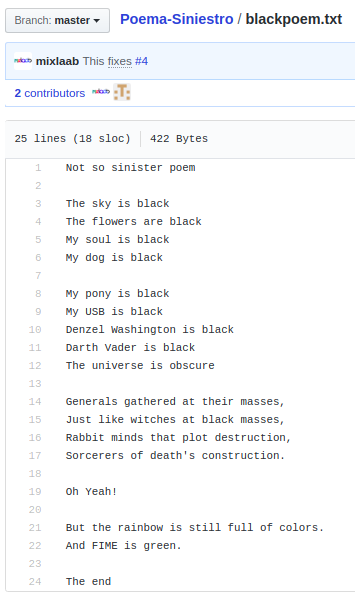
\includegraphics [scale=0.33]{step1}
%\caption{Sección de Issues}
\label{fig:step1}
\end{figure}
    
\end{block}
\end{frame}

%\section{Merge conflicts}

\begin{frame}{Colaboración entre usuarios}{Poema Siniestro}

\begin{block}{Lista de pull requests en mi poema}

\begin{figure}[h!]
\centering

\includegraphics [scale=0.27]{step2}
%\caption{Sección de Issues}
\label{fig:step2}
\end{figure}
\vspace{-0.2in}
\begin{figure}[h!]
  \centering
  
\includegraphics [scale=0.27]{step2_1}
  %\caption{Sección de Issues}
  \label{fig:step2_1}
\end{figure}

\end{block}

\end{frame}

\section{Poeta Fimeño}

\begin{frame}{Poeta Fimeño}{Usuario inspirado}

\begin{block}{Premio al mejor poema (Cuenta: jorgejlmh)}

\begin{figure}[h!]
\centering
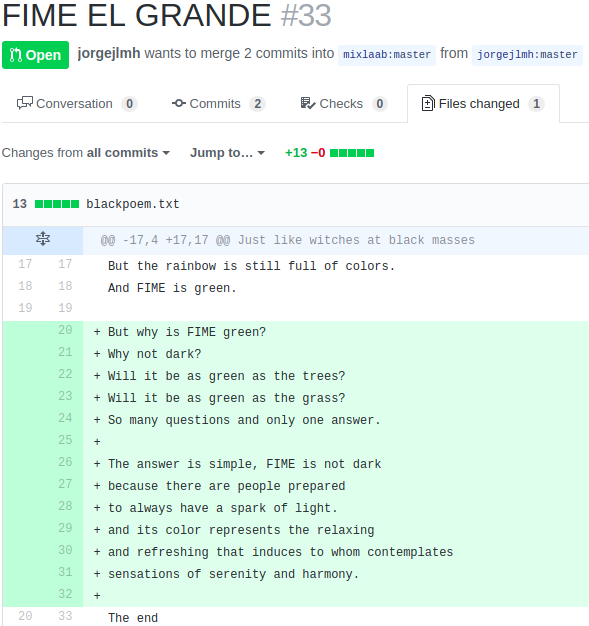
\includegraphics [scale=0.28]{step3}
%\caption{Sección de Issues}
\label{fig:step3}
\end{figure}
    
\end{block}

\end{frame}

\begin{frame}{Creando y borrando remotos}{Desde la terminal}

  \begin{block}{Clonando un remoto}
  
  \begin{figure}[h!]
  \centering
  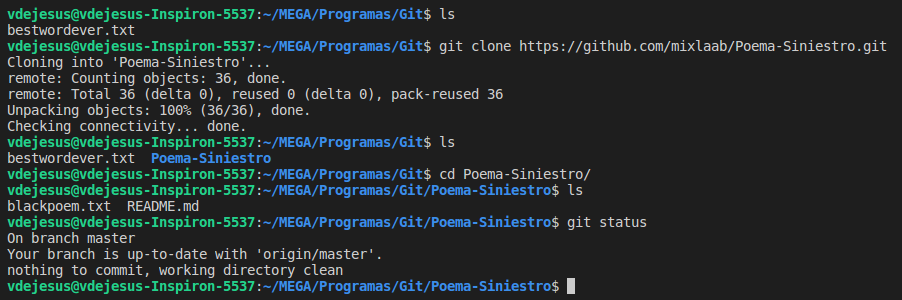
\includegraphics [scale=0.3]{step4}
  %\caption{Sección de Issues}
  \label{fig:step4}
  \end{figure}
      
  \end{block}
  
\end{frame}

\begin{frame}{Creando y borrando remotos}{Desde la terminal}

  \begin{block}{Borrando un remoto y creando otro con nuevo nombre}
  
  \begin{figure}[h!]
  \centering
  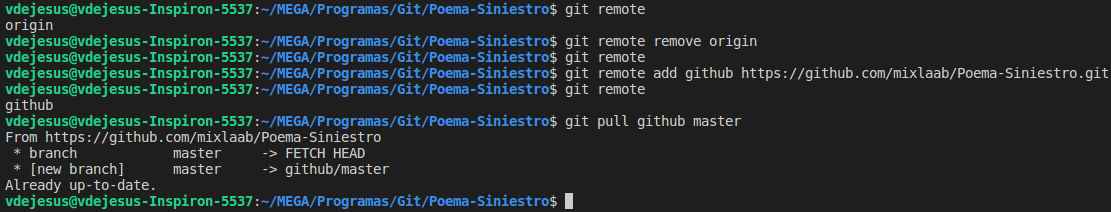
\includegraphics [scale=0.24]{step5}
  %\caption{Sección de Issues}
  \label{fig:step5}
  \end{figure}
      
  \end{block}
  
\end{frame}

\begin{frame}{Creando y borrando remotos}{Desde la terminal}

  \begin{block}{Vamos al repo del usuario que hizo pull request}
  
  \begin{figure}[h!]
  \centering
  
\includegraphics [scale=0.34]{step6}
  %\caption{Sección de Issues}
  \label{fig:step6}
  \end{figure}
      
  \end{block}
  
\end{frame}

\begin{frame}{Creando y borrando remotos}{Desde la terminal}

  \begin{block}{Copiamos enlace del repo}
  
  \begin{figure}[h!]
  \centering
  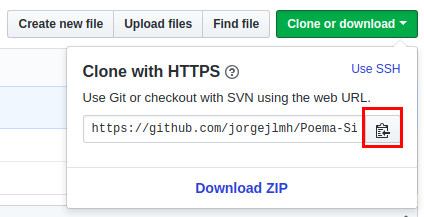
\includegraphics [scale=0.4]{step7}
  %\caption{Sección de Issues}
  \label{fig:step7}
  \end{figure}
      
  \end{block}
  
\end{frame}

\begin{frame}{Creando y borrando remotos}{Desde la terminal}

  \begin{block}{Añadimos el repo del usuario como remoto}
  
  \begin{figure}[h!]
  \centering
  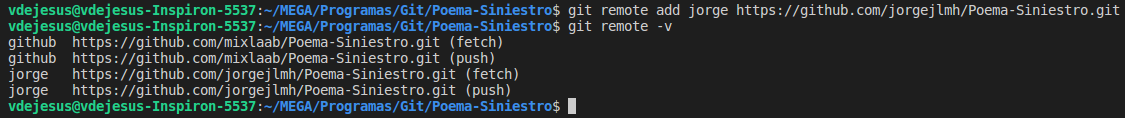
\includegraphics [scale=0.25]{step8}
  %\caption{Sección de Issues}
  \label{fig:step8}
  \end{figure}
      
  \end{block}
  
\end{frame}

\begin{frame}{Creando y borrando remotos}{Desde la terminal}

  \begin{block}{Pull Request + Merge (Local)}
  
  \begin{figure}[h!]
  \centering
  
\includegraphics [scale=0.38]{step9}
  %\caption{Sección de Issues}
  \label{fig:step9}
  \end{figure}
      
  \end{block}
  
\end{frame}

\begin{frame}{Verificando cambios en el repositorio local}{Desde la terminal}

  \begin{block}{Contenido del archivo local}
  
  \begin{figure}[h!]
  \centering
  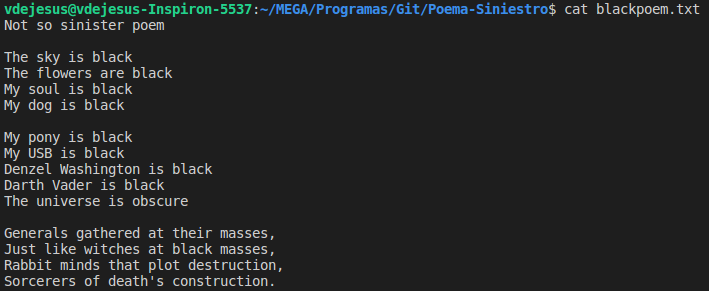
\includegraphics [scale=0.4]{step10}
  %\caption{Sección de Issues}
  \label{fig:step10}
  \end{figure}
      
  \end{block}
  
\end{frame}

\begin{frame}{Verificando cambios en el repositorio local}{Desde la terminal}

  \begin{block}{Contenido del archivo local}
  
  \begin{figure}[h!]
  \centering
  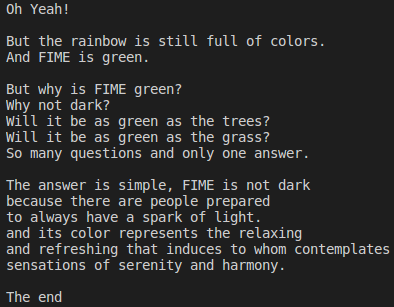
\includegraphics [scale=0.4]{step11}
  %\caption{Sección de Issues}
  \label{fig:step11}
  \end{figure}
      
  \end{block}
  
\end{frame}

\begin{frame}{Pasando cambios al remoto}{Desde la terminal}

  \begin{block}{Si checamos el repositorio remoto veremos que aun no está actualizado}
  
  \begin{figure}[h!]
  \centering
  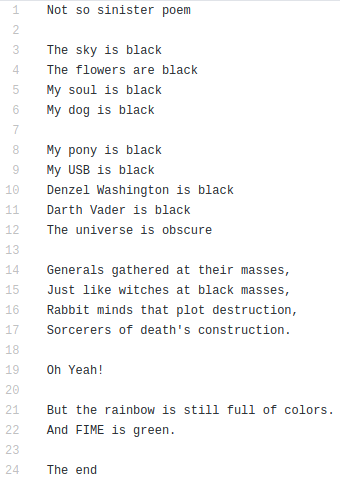
\includegraphics [scale=0.28]{step11_2}
  %\caption{Sección de Issues}
  \label{fig:step11_2}
  \end{figure}
      
  \end{block}
  
\end{frame}

\begin{frame}{Pasando cambios al remoto}{Desde la terminal}

  \begin{block}{Falta hacer merge en remoto}
  Pero antes agregaremos un comentario a la persona que solicita el pull request. Usaremos terminal para hacer el merge en vez de dar clic en el botón verde.
  \begin{figure}[h!]
  \centering
  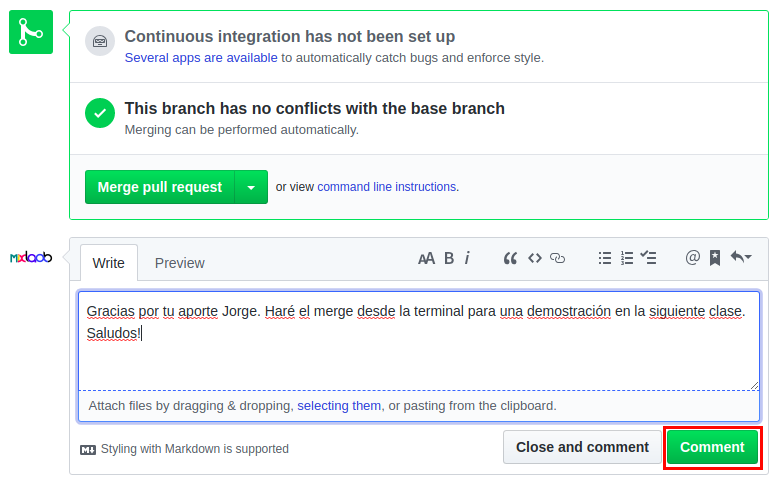
\includegraphics [scale=0.28]{step12}
  %\caption{Sección de Issues}
  \label{fig:step12}
  \end{figure}
      
  \end{block}
  
\end{frame}

\begin{frame}{Titulo}{}

  \begin{block}{}
  
  \begin{figure}[h!]
  \centering
  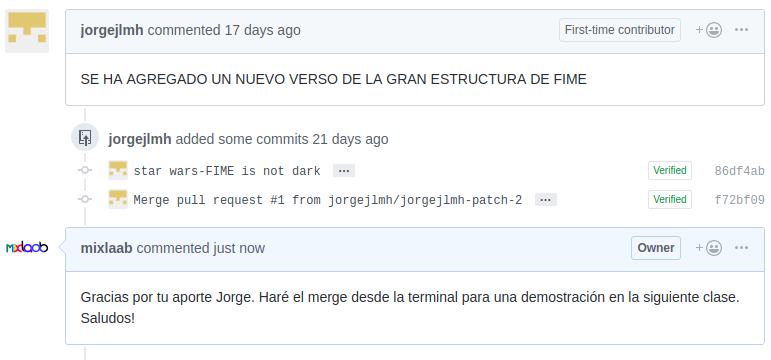
\includegraphics [scale=0.28]{step13}
  %\caption{Sección de Issues}
  \label{fig:step13}
  \end{figure}
      
  \end{block}
  
\end{frame}

\begin{frame}{Titulo}{}

  \begin{block}{}
  
  \begin{figure}[h!]
  \centering
  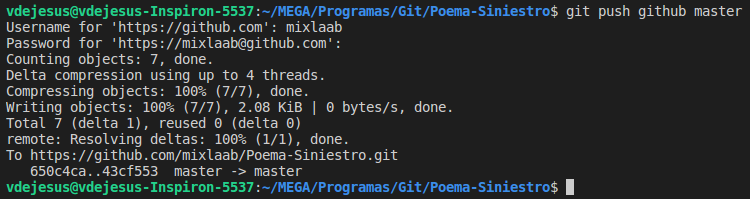
\includegraphics [scale=0.28]{step14}
  %\caption{Sección de Issues}
  \label{fig:step14}
  \end{figure}
      
  \end{block}
  
\end{frame}

\begin{frame}{Titulo}{}

  \begin{block}{}
  
  \begin{figure}[h!]
  \centering
  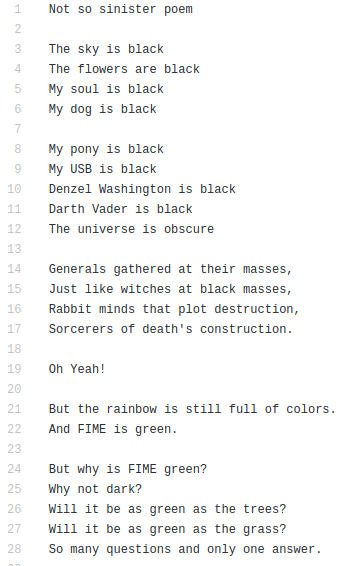
\includegraphics [scale=0.28]{step15}
  %\caption{Sección de Issues}
  \label{fig:step15}
  \end{figure}
      
  \end{block}
  
\end{frame}

\begin{frame}{Titulo}{}

  \begin{block}{}
  
  \begin{figure}[h!]
  \centering
  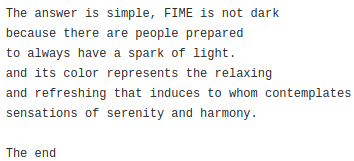
\includegraphics [scale=0.28]{step15_2}
  %\caption{Sección de Issues}
  \label{fig:step15_2}
  \end{figure}
      
  \end{block}
  
\end{frame}

\begin{frame}{Titulo}{}

  \begin{block}{}
  
  \begin{figure}[h!]
  \centering
  
\includegraphics [scale=0.28]{step16}
  %\caption{Sección de Issues}
  \label{fig:step16}
  \end{figure}
      
  \end{block}
  
\end{frame}

\section{Información de contacto}
% contact information
\begin{frame}{Feedback}{Información de contacto}
En caso de comentarios, sugerencias, preguntas o errores en las diapositivas no dudes en contactarme.
  \begin{center}
    \insertauthor\\
    \chref{https://mixlaab.github.io}{https://mixlaab.github.io}\\
    WA: 8119022700\\
    %9220 Aalborg Ø
  \end{center}
\end{frame}
%%%%%%%%%%%%%%%%

{\aauwavesbg%
\begin{frame}[plain,noframenumbering]%
  \finalpage{Fin}
\end{frame}}
%%%%%%%%%%%%%%%%

\end{document}
